\documentclass[border=8pt,tikz]{standalone}
\usepackage{tikz}
% Shared TikZ style for Chapter 5 diagrams.
% Inputted by every standalone diagram file.

\usetikzlibrary{
  arrows.meta,
  positioning,
  shapes.geometric,
  shapes.symbols,
  shapes.multipart,
  shapes.misc,
  fit,
  calc,
  backgrounds,
  decorations.pathmorphing,
  decorations.pathreplacing,
  patterns,
  shadows.blur,
}

% ─── Colour palette ──────────────────────────────────────────────
\definecolor{strixBlue}{HTML}{3B7DD8}     % data sources / inputs
\definecolor{strixGreen}{HTML}{22A699}    % processing / workers
\definecolor{strixOrange}{HTML}{E08036}   % storage
\definecolor{strixRed}{HTML}{E04B4B}      % attacker / external threat
\definecolor{strixPurple}{HTML}{6B5DD3}   % frontend / UI
\definecolor{strixGold}{HTML}{F2BE22}     % models / ML
\definecolor{strixGrey}{HTML}{6E7681}     % neutral / labels
\definecolor{strixDark}{HTML}{1F2933}     % titles / borders

% ─── Common node styles ──────────────────────────────────────────
\tikzset{
  >={Latex[width=2mm,length=2.5mm]},
  font=\sffamily\small,
  every node/.style={align=center},
  comp/.style={
    rectangle, rounded corners=2pt, draw=#1, fill=#1!10, very thick,
    text=strixDark, minimum width=22mm, minimum height=8mm,
    inner sep=4pt,
  },
  comp/.default=strixGreen,
  store/.style={
    cylinder, shape border rotate=90, aspect=0.3, draw=strixOrange,
    fill=strixOrange!12, very thick, text=strixDark,
    minimum width=18mm, minimum height=10mm, inner sep=2pt,
  },
  stream/.style={
    rectangle, rounded corners=2pt, draw=strixOrange,
    fill=strixOrange!8, dashed, thick, text=strixDark,
    minimum width=22mm, minimum height=7mm, inner sep=3pt,
    font=\ttfamily\scriptsize,
  },
  source/.style={comp=strixBlue},
  worker/.style={comp=strixGreen},
  model/.style={comp=strixGold},
  ui/.style={comp=strixPurple},
  ext/.style={comp=strixRed},
  title/.style={font=\sffamily\bfseries, text=strixDark},
  edge/.style={->, thick, draw=strixGrey, font=\sffamily\scriptsize\itshape},
  edgeStrong/.style={->, very thick, draw=strixDark, font=\sffamily\scriptsize\bfseries},
  group/.style={
    rectangle, rounded corners=4pt, draw=strixGrey, dashed, thick,
    inner sep=6pt, fill=strixGrey!4,
  },
  badge/.style={
    rectangle, rounded corners=1pt, fill=#1, text=white,
    font=\sffamily\scriptsize\bfseries, inner sep=2pt,
  },
  badge/.default=strixDark,
  port/.style={
    rectangle, rounded corners=1pt, draw=strixDark, fill=strixGrey!8,
    font=\ttfamily\scriptsize, minimum width=14mm, inner sep=2pt,
  },
}


\begin{document}
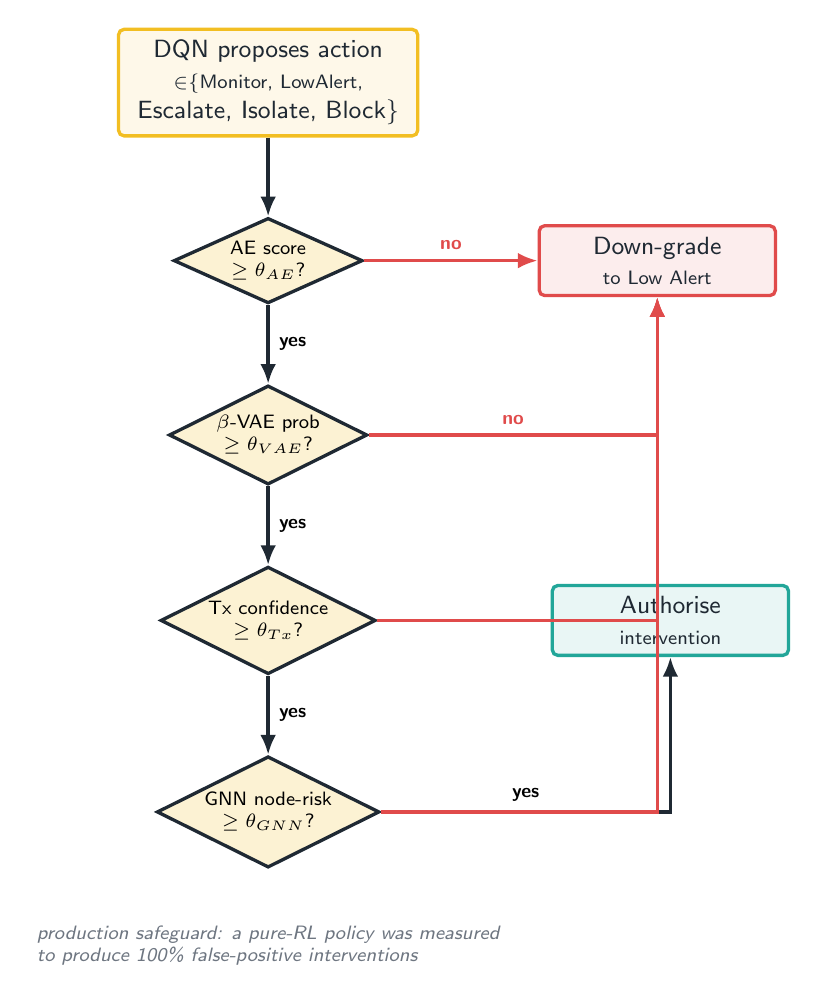
\begin{tikzpicture}[node distance=10mm,
  decision/.style={diamond, draw=strixDark, fill=strixGold!20, very thick,
                   aspect=2, inner sep=1pt, font=\sffamily\scriptsize, align=center,
                   minimum width=24mm},
  action/.style={comp=strixGreen, minimum width=30mm}]

\node[model, minimum width=38mm] (dqn) {DQN proposes action\\\scriptsize\(\in\)\{Monitor, LowAlert,\\Escalate, Isolate, Block\}};

\node[decision, below=of dqn] (g1) {AE score\\\(\geq\theta_{AE}\)?};
\node[decision, below=of g1] (g2) {$\beta$-VAE prob\\\(\geq\theta_{VAE}\)?};
\node[decision, below=of g2] (g3) {Tx confidence\\\(\geq\theta_{Tx}\)?};
\node[decision, below=of g3] (g4) {GNN node-risk\\\(\geq\theta_{GNN}\)?};

\node[action, right=22mm of g3] (auth) {Authorise\\\scriptsize intervention};
\node[action, fill=strixRed!10, draw=strixRed, right=22mm of g1] (down) {Down-grade\\\scriptsize to Low Alert};

\draw[edgeStrong] (dqn) -- (g1);
\draw[edgeStrong] (g1) -- (g2) node[midway, right, font=\sffamily\scriptsize\bfseries] {yes};
\draw[edgeStrong] (g2) -- (g3) node[midway, right, font=\sffamily\scriptsize\bfseries] {yes};
\draw[edgeStrong] (g3) -- (g4) node[midway, right, font=\sffamily\scriptsize\bfseries] {yes};
\draw[edgeStrong] (g4) -| (auth) node[near start, above, font=\sffamily\scriptsize\bfseries] {yes};

\draw[edgeStrong, draw=strixRed] (g1.east) -- (down) node[midway, above, font=\sffamily\scriptsize\bfseries, text=strixRed] {no};
\draw[edgeStrong, draw=strixRed] (g2.east) -| (down) node[near start, above, font=\sffamily\scriptsize\bfseries, text=strixRed] {no};
\draw[edgeStrong, draw=strixRed] (g3.east) -| (down);
\draw[edgeStrong, draw=strixRed] (g4.east) -| (down);

\node[font=\sffamily\scriptsize\itshape, text=strixGrey, anchor=north, align=left]
  at ([yshift=-6mm]g4.south)
  {production safeguard: a pure-RL policy was measured\\to produce 100\% false-positive interventions};

\end{tikzpicture}
\end{document}
